\par
Notre application utilise le script jquery-qrcode\footnote{https://larsjung.de/jquery-qrcode/} pour générer les images des QR Codes. Il a l'avantage d'être très souple d'utilisation et de pouvoir générer des QR Codes aux formats assez complexes. Il permet notamment d'insérer une image ou un champ texte au QR Code, ainsi que de définir les couleurs du texte central et du QR Code. Nous avons tiré profit de ces caractéristiques pour laisser la possibilité aux transcripteurs de l'institut d'insérer un texte en braille central, d'une couleur pouvant être imprimée en relief (LIEN INTRO/OBJECTIFS). Un QR Code de type atomique (REF TYPES QR) possédant des caractères centraux en braille est visible ci-dessous.\\

\begin{figure}[]
	\centering
   
\includegraphics[scale=0.25]{img/qrsimple.jpeg}
   \caption{QR Code simple}
\end{figure}

\par
La génération des images est effectuée par la classe du Contrôleur \classe{ImageGenerator} (LIEN ARCHITECTURE). En plus des QR Codes simples, elle permet de générer des images de sauvegarde des familles de QR Codes (LIEN TYPES QR et LIEN CHARGEMENT QR). Ces images contiennent le contenu des QR Codes de la famille dans les métadonnées, et des informations sur la famille imprimées sur l'image. Un exemple d'une image famille générée par l'application est visible ci-dessous.

\begin{figure}[]
	\centering
   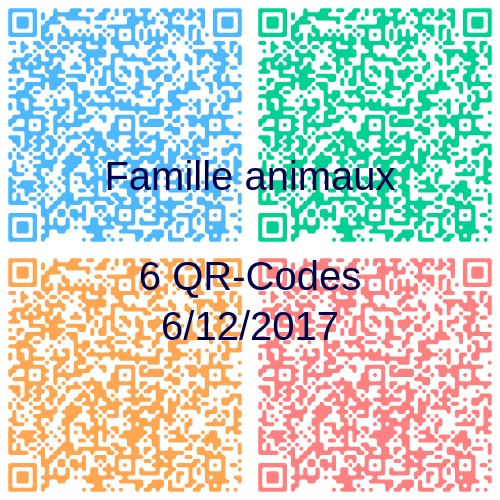
\includegraphics[scale=0.2]{img/animaux.jpeg}
   \caption{Image de sauvegarde famille}
\end{figure}